\documentclass[a4paper]{article}

\usepackage[english]{babel}
\usepackage[utf8]{inputenc}
\usepackage{amsmath}
\usepackage{graphicx}
\usepackage{indentfirst}


%opening
\title{Pricom - Exercício de Simulação nº01\\Turma A}
\author{Filipe Miguel\\
	Lucas Siqueira}

\begin{document}

\maketitle


\section{Procedimentos}
\subsection*{Parte 1 – Compreendendo a DFT}
	O objetivo da parte 1 deste relatório é entender o cálculo numérico da Transformada de Fourier. Para isso devemos ter em mente o cálculo de acordo com o número discreto de frequências escolhidas. Por vezes, recairmos em sinais não limitados no tempo e para isso, é necessário truncá-lo para que tenha duração finita.

		\begin{enumerate} 
			\item Gerar um sinal $x(t) = cos(2\pi f_1t)-sin(2\pi f_11)$ com $f_1=1$Hz e $f_2 = 1.5$Hz. Taxa de amostragem de 20Hz.
			\begin{figure}[!hb]
				\centering
				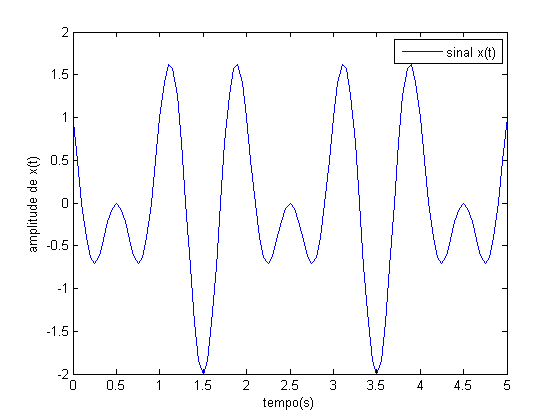
\includegraphics[scale=0.5]{fig1.png}
				\caption{Gráfico de $x(t)$}
				\label{fig1}
			\end{figure}
			\item Calculo da DFT do sinal utilizando o tempo de duração $T_0 = 5s$ e número de pontos dado por $N = \frac{Ts}{T_0}$. Vale observar que a escolha do padrão de utilizar a próxima potência de 2 no cálculo da variável NFFT dar-se-a pela simples manipulação do algoritmo imposto dentro da função FFT (\textit{Fast Fourier Transform}). 
			\begin{figure}[!h]
				\centering
				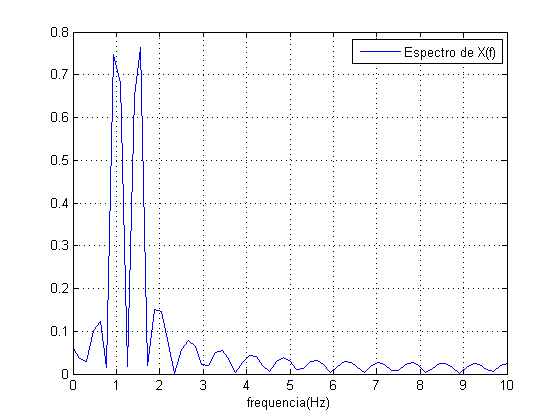
\includegraphics[scale=0.5]{fig2.png}
				\caption{Espectro de $X(f)$}
				\label{fig2}
			\end{figure}
			\begin{figure}[!hr]
				\centering
				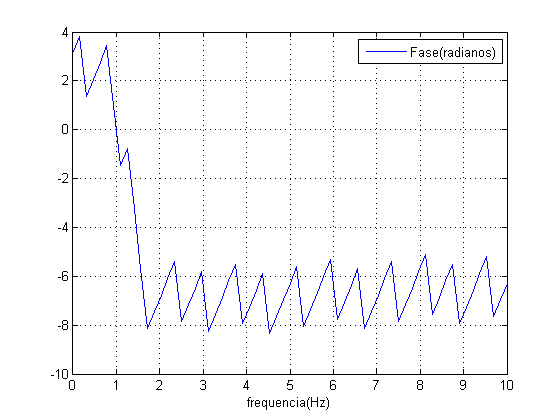
\includegraphics[scale=0.5]{fig3.png}
				\caption{Fase de $X(f)$}
				\label{fig3}
			\end{figure}
			Conforme observado no gráfico acima observamos dois lóbulos formados em tornos das frequências fundamentais do sinal x(t), a saber, 1Hz e 1.5Hz. O que difere um pouco do esperado pela transformada teórica que seria observado dois impulsos em torno dessas frequências.
			\item Repetindo os itens 1.1 e 1.2 temos os seguintes gráficos para um intervalo de duração de 20 segundos:
			\begin{figure}[!hr]
				\centering
				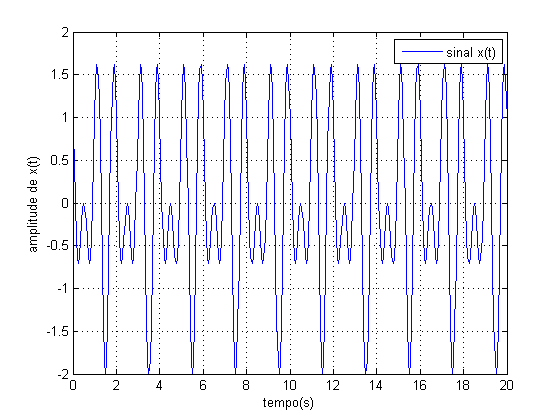
\includegraphics[scale=0.5]{fig4.png}
				\caption{Sinal de $x(t)$}
				\label{fig4}
			\end{figure}
			\begin{figure}[!hl]
				\centering
				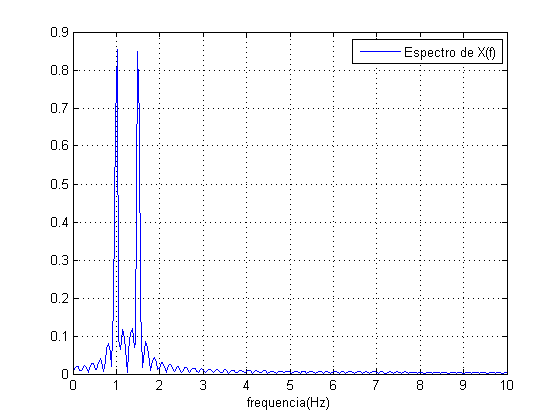
\includegraphics[scale=0.5]{fig5.png}
				\caption{Espectro de $X(f)$}
				\label{fig5}
			\end{figure}
			\begin{figure}[!hr]
				\centering
				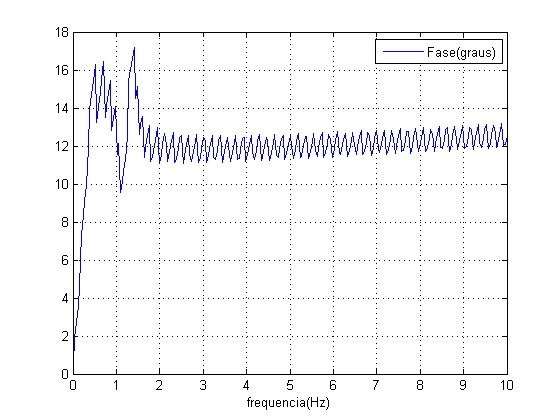
\includegraphics[scale=0.5]{fig6.png}
				\caption{Espectro de $X(f)$}
				\label{fig6}
			\end{figure}
			\item Utilizando uma amostra menor com $fa1 = 5Hz$ e $fa2 = 2Hz.$ Temos os seguintes resultados:
			\begin{figure}[!hr]
				\centering
				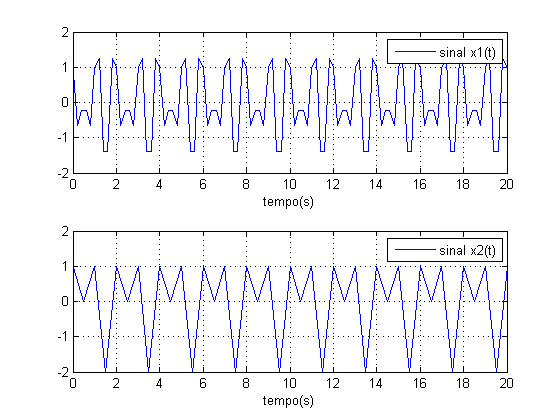
\includegraphics[scale=0.5]{fig7.png}
				\caption{Sinais de $x1(t)$ e $x2(t)$}
				\label{fig7}
			\end{figure}
			\begin{figure}[!hl]
				\centering
				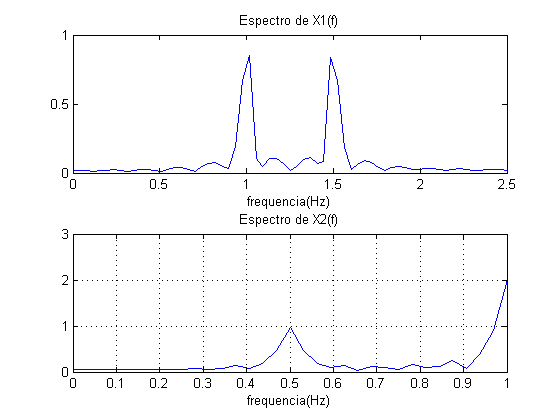
\includegraphics[scale=0.5]{fig8.png}
				\caption{Espectros dos sinais}
				\label{fig8}
			\end{figure}
			\begin{figure}[!hr]
				\centering
				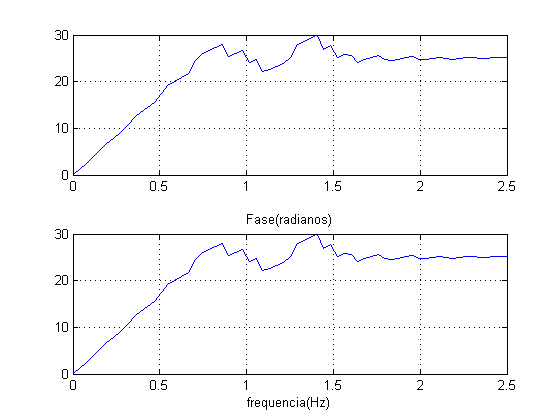
\includegraphics[scale=0.5]{fig9.png}
				\caption{Fase dos sinais}
				\label{fig9}
			\end{figure}
			No caso para frequência de amostragem B = 2Hz ou seja fa necessariamente tem que ser maior que 2B ou seja fa maior que 4Hz. Dessa forma na figura \ref{fig8} houve o fenômeno de dobramento espectral.
		\end{enumerate}
\subsection{Parte 2 - Densidade Espectral de Potência e Filtros}
	O carregamento de imagem foi dada conforme o código anexo Q2.m utilizando algumas funções disponíveis no software \textit{MATLAB}.
	\begin{figure}[!hr]
		\centering
		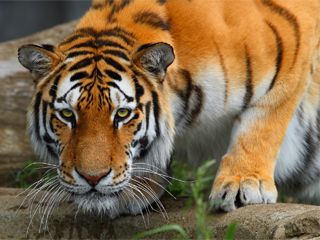
\includegraphics[scale=0.5]{sample.png}
		\caption{Imagem de amostra}
		\label{sample1}
	\end{figure}
	Gráfico da figura amostrada.
	\begin{figure}[!hr]
		\centering
		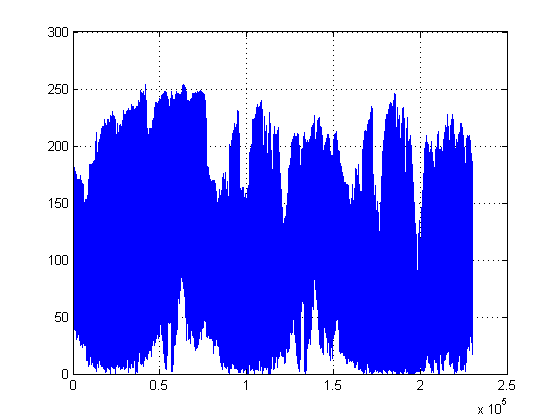
\includegraphics[scale=0.5]{fig21.png}
		\caption{Sinal amostrado}
		\label{sample2}
	\end{figure}
	Grafico plotado considerando a autocorrelação de sinal.
	\begin{figure}[!hr]
		\centering
		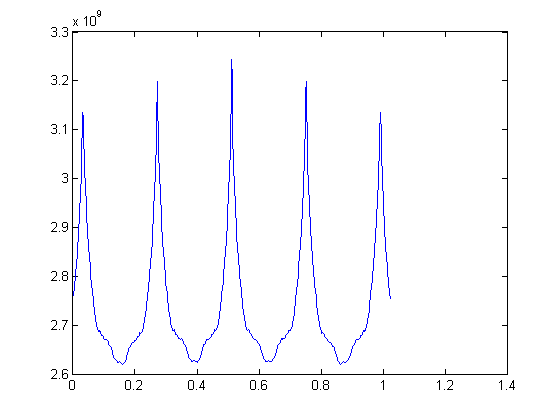
\includegraphics[scale=0.5]{fig22.png}
		\caption{Imagem de amostra}
		\label{sample3}
	\end{figure}
	



\subsection{Parte 3 – Modulação Analógica}
\end{document}
